\documentclass[tikz,border=3mm]{standalone}

\begin{document}

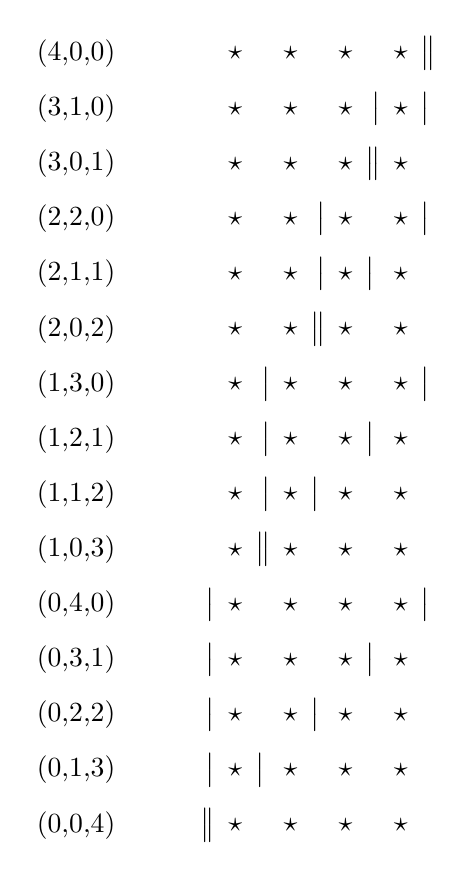
\begin{tikzpicture}[scale=.7]
  \def\total{4} % i+j+k = total
  \xdef\y{0}
  \foreach \i in {0,...,\total}{
    \pgfmathsetmacro{\maxj}{int(\total-\i)}
    \foreach \j in {0,...,\maxj}{
      \pgfmathparse{int(\y+1)}\xdef\y{\pgfmathresult}
      \pgfmathsetmacro{\k}{int(\total-\i-\j)}
      \foreach \i in {1,...,\total}
        \node at (\i,\y){$\star$};
      \node at (.45+\j+\i,\y) {$\big|$};
      \node at (.55+\i,\y) {$\big|$};
      \node[left] at (-1,\y){(\i,\j,\k)};
    }
  }
\end{tikzpicture}

\end{document}
